%! Author = bytelai
%! Date = 2021/12/24

% Preamble
\documentclass[UTF8]{ctexart}

% Packages
\usepackage{amsmath}
\usepackage{amsfonts}
\usepackage{textcomp}
\usepackage{graphicx}
\usepackage{url}
\usepackage{algorithm}
\usepackage{subfigure}
\usepackage{algorithmic}
\usepackage{bm}
\usepackage{natbib}
\usepackage{siunitx}
\usepackage{mathrsfs}
\usepackage{amssymb}
\newcommand{\myciteup}[1]{\textsuperscript{\textsuperscript{\cite{#1}}}}
%\usepackage[textwidth=14.5cm]{geometry}
%\usepackage{blindtext}
%\parindent=0pt
\title{工作日志}
\author{lwj}

% Document
\begin{document}

    \begin{sloppypar}
        \maketitle
        \newpage
        \tableofcontents
        \newpage
        \section{wildDfd论文阅读}
        \subsection{wildDFD}
        wild DFD\myciteup{2017Depth}的算法框架如图\ref{fig:wild:framework},通过建立目标函数,设计相关优化算法,进行求解深度信息。其特点是两帧的模糊图像之间可以有相对运动的存在(算法中设计了光流估计环节进行补偿),算法分为两个过程,$top-down likelihood$和$bottom-up likelihood$,其中$top-down likelihood$通过对图像进行分割,利用分割信息对后续的深度补全提供线索信息,建立损失函数$E_{DFD}$。$bottom-up likelihood$将图像分为多个块(patch),在每个块内,利用对均衡滤波模型\myciteup{2006Depth}进行改进,建立优化模型,求解得到深度信息,在通过局部的平滑先验建立损失函数$E_{prior}$。对于建立好的模型,通过求解马尔科夫随机场问题和二次型问题,对深度进行求解。
        \begin{figure}[htbp]
            \centering
            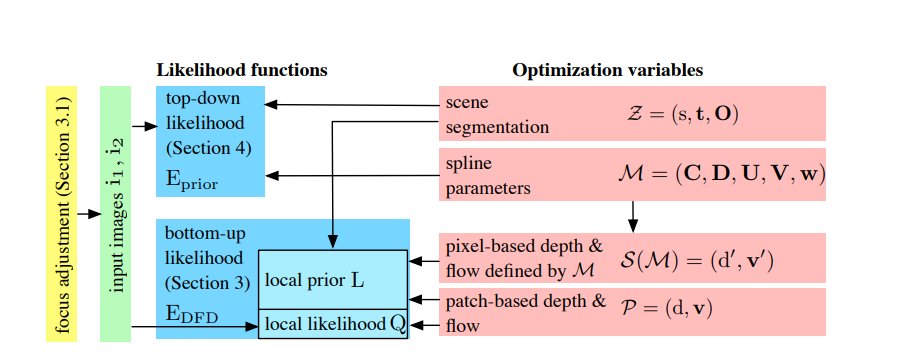
\includegraphics[width=0.9\linewidth]{figure/wildDfdFramework}
            \caption{\small wildDfd算法框架\myciteup{2017Depth}}
            \label{fig:wild:framework}
        \end{figure}
        \section{用于图像分割的特征提取}
        \subsection{Bilateral Affinity Matrix}
        双边仿射矩阵$S$的元素$S(p,q)$表征的是图像不同位置$p$和$q$之间的关联性。其中其中$p$和$q$可以理解成将图像张成向量之后的坐标。$S$的拉普拉斯矩阵对应的的特征向量,可以包含一定的图像分割信息。相似性通过式\eqref{eq:S}\eqref{eq:Delta}建立\myciteup{2017Depth},其中$l,a,b$是图像$LAB$色域内的三通道信息,
        \begin{equation}
            S(p,q)=\left \{
            \begin{array}{cc}
                exp(-\Delta_{pq})+exp(-\Delta_{qp}) \ \ if \left | p - q  \right | <3\sigma_s\\
                0&, others\\
            \end{array} \right.
            \label{eq:S}
        \end{equation}
        \begin{equation}
            \Delta_{pq} = min(\frac{\left | l_p - l_q \right |^2}{2\sigma_{pl}^2} +
            \frac{\left | a_p - a_q \right |^2}{2\sigma_{pa}^2} +
            \frac{\left | b_p - b_q \right |^2}{2\sigma_{pb}^2},\epsilon) +
            \frac{\left | p-q\right |^2}{2\sigma_{s}^2}
            \label{eq:Delta}
        \end{equation}
        $S$ 的拉普拉斯矩阵如下:
        \begin{equation}
            L = Diag(sum_{per col}(S)) - S
            \label{eq:L}
        \end{equation}
        \subsection{DNCuts}
        仿射矩阵$S$的拉普拉斯矩阵$L$(见\eqref{eq:L})是一个超高维的矩阵,其特征值的计算复杂度很高,因此Arbelaez\myciteup{2014Multiscale}提出了DNCuts算法进行优化求解。DNCuts算法基于以下的知识:
        \begin{itemize}
            \item 如果$S$按行或者按列求和为1,则$S$和$S^2$的拉普拉斯矩阵的特征向量是相等的。
            \item 对$S$进行降采样(隔行丢或者隔列丢)后求解特征向量近似于对$S$的特征向量进行降采样。
        \end{itemize}
        直接对$S$进行降采样效果不理想,因此对$S^2$进行降采样。Arbelaez\myciteup{2014Multiscale}给出的解释是,通过计算$S^{T}S$,$S^2$的每一列都包含了其他列的信息。因此降采样不会造成太多的信息丢失。计算得到的结果如图\ref{fig:DNCuts},可以看出拉普拉斯仿射矩阵的特征值和图像分割具有相关性。
        \begin{figure}[htbp]
            \centering
            \subfigure[30个特征值图像]{
                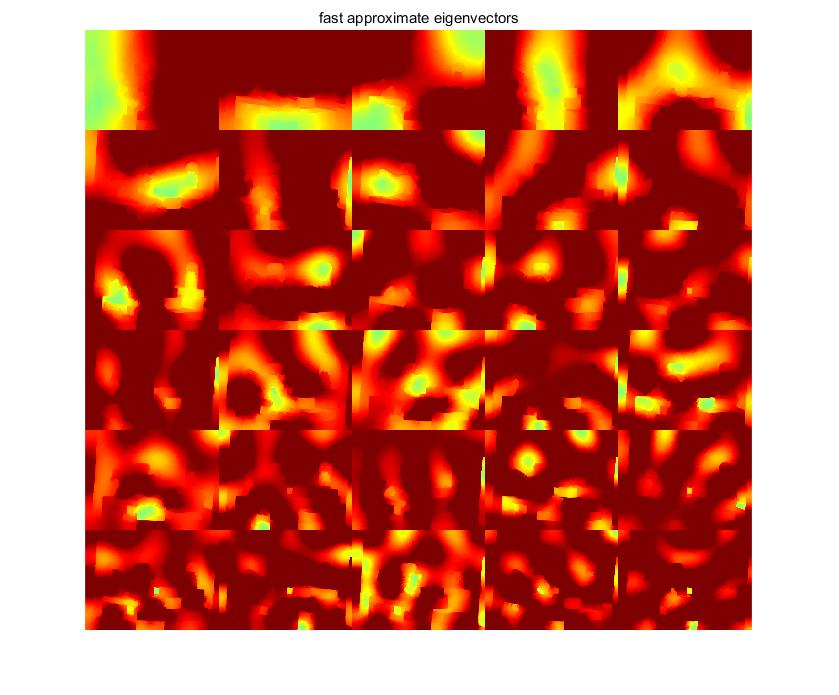
\includegraphics[width=0.45\linewidth]{figure/DNCutsZebraEig}}
            \quad
            \subfigure[特征值融合之后的伪彩图]{
                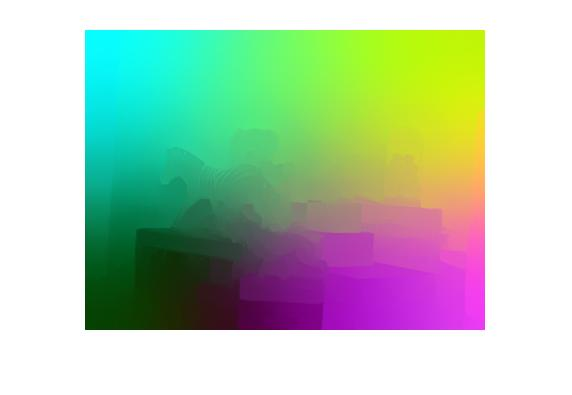
\includegraphics[width=0.45\linewidth]{figure/DNCutsZebraPseudoColor}}
            \quad
            \caption{\small DNCuts算法计算图像分割特征}
            \label{fig:DNCuts}
        \end{figure}
        \section{基于模糊均衡的DFD技术}
        \subsection{S Transform}
        Spatial-doman convolution/Deconvolution Transform\myciteup{subbarao1991spatial}简称(S Transform)技术,是一种计算多项式卷积和去卷积的快速算法。图像可以利用三次二维的多项式\eqref{eq:Imgpoly}进行拟合
        \begin{equation}
            f(x,y) = \sum\limits_{m=0}^{3}\sum\limits_{n=0}^{3}a_{mn}x^my^n
            \label{eq:Imgpoly}
        \end{equation}
        记$h(x,y)$为旋转对称的点扩散函数(PSF),相应的模糊退化模型为\eqref{eq:blur},其中$\ast$ 表示卷积
        \begin{equation}
            g(x,y) = f(x,y)\ast h(x,y)
            \label{eq:blur}
        \end{equation}
        如式\eqref{eq:psfSigma}所示,对于旋转不变的PSF,可以用参数$\sigma_h$进行表征,
        \begin{equation}
            \sigma_h^2 = \iint_{-\infty}^{+\infty}(x^2+y^2)h(x,y)dxdy
            \label{eq:psfSigma}
        \end{equation}
        利用S变换\myciteup{subbarao1991spatial}可得,其去卷积(deconvolution)过程可以用式\eqref{eq:STMDecon}表示,其中$\nabla^2$为拉普拉斯算子,式\eqref{eq:STMDecon}也经常用来进行图像边缘的增强
        \begin{equation}
            f(x,y) = g(x,y) - \frac{\sigma_h^2}{4}\nabla^{2}g(x,y)
            \label{eq:STMDecon}
        \end{equation}
        对于利用两种对焦参数拍摄的图像,其点扩散函数的参数$\sigma_1,\sigma_2$的关系如式\eqref{eq:stsigmaVssigma},$\alpha$表征两幅图像的放大率变化:
        \begin{equation}
            \sigma_1 = \alpha\sigma_2 + \beta
            \label{eq:stsigmaVssigma}
        \end{equation}
        由\eqref{eq:STMDecon}可以得到:
        \begin{equation}
            g_1 - g_2 = \frac{1}{4}G\nabla^{2}g
            \label{eq:st_g1_g2}
        \end{equation}
        其中
        \begin{equation}
            \nabla^{2} = \nabla^{2}g1=\nabla^2 g2
            \label{eq:stDg1EqDg2}
        \end{equation}
        可以得到
        \begin{equation}
            G=\sigma_1^2-\sigma_2^2 = \frac{4(g_1-g_2)}{\nabla^2 g}
            \label{eq:stG}
        \end{equation}
        代入式\eqref{eq:stsigmaVssigma}得到
        \begin{equation}
            \sigma_2^2(\alpha^2-1)+2\alpha\beta\sigma_2+\beta^2 = G
            \label{eq:stSigma2G}
        \end{equation}
        如果放大率不变也即$\alpha=1$,则式\eqref{eq:stSigma2G}可以写成
        \begin{equation}
            \sigma_2 = \frac{G}{2\beta} - \frac{\beta}{2}
            \label{eq:stSigma2G_2}
        \end{equation}
        利用式\eqref{eq:STMDecon}进行去卷积会放大图像的高频部分,进而降低信噪比,同时\eqref{eq:st_g1_g2}要求$\nabla^{2} = \nabla^{2}g1=\nabla^2 g2$(对于理想的二维三次多项式模型的STM变换,成立\myciteup{subbarao1991spatial}),实际的图像由于噪声的影响,式\eqref{eq:stDg1EqDg2}很难成立。因此Xian等提出了BET方法来替代STM进行深度估计\myciteup{2006Depth}。
        通过将两张模糊图像分别和适当的PSF(可以已知高频噪声)进行卷积,进一步的,通过BET可以减少对式\eqref{eq:stDg1EqDg2}的依赖。对$g_1,g_2$分别用各自的卷积核$h_1,h_2$进行卷积。得到式\eqref{eq:stG1h2_G2h1}
        \begin{equation}
            \begin{array}{cc}
                g_1(x,y) \ast h_2(x,y) &= \left[ f(x,y) \ast h_1(x,y) \right]\ast h_2(x,y)\\
                g_2(x,y) \ast h_1(x,y) &= \left[ f(x,y) \ast h_2(x,y) \right]\ast h_1(x,y)\\
            \end{array}
            \label{eq:stG1h2_G2h1}
        \end{equation}
        由卷积运算的交换性可以得到
        \begin{equation}
            g_1(x,y)\ast h_2(x,y) = g_2(x,y) \ast h_1(x,y)
            \label{eq:stG1h2EqG2h1}
        \end{equation}
        利用STM前向变换计算卷积得到:
        \begin{equation}
            \begin{array}{cc}
                g_1(x,y)\ast h_2(x,y) &= g_1(x,y) + \frac{\sigma_2 ^2}{4}\nabla^2 g_1(x,y) + \frac{\sigma_2 ^4}{24}(\nabla ^2)^{2}g_1(x,y) +R(O^6)\\
                g_2(x,y)\ast h_1(x,y) &= g_2(x,y) + \frac{\sigma_1 ^2}{4}\nabla^2 g_2(x,y) + \frac{\sigma_1 ^4}{24}(\nabla ^2)^{2}g_2(x,y) +R(O^6)\\
            \end{array}
            \label{eq:g2h1StmForward}
        \end{equation}
        省去高阶项($R(O^4,O^6)$),可得
        \begin{equation}
            g_1(x,y) + \frac{\sigma_2^2}{4}\nabla ^2 g_1(x,y) = g_2(x,y) + \frac{\sigma_1^2}{4}\nabla^{2}g_2(x,y)
            \label{eq:stg1vsg2}
        \end{equation}
        结合式\eqref{eq:stsigmaVssigma},可以得到
        \begin{equation}
            a_1\sigma_1 ^2 + b_1 \sigma_1 +c_1 = 0
            \label{eq:stSigma1Module}
        \end{equation}
        其中
        \begin{equation}
            \begin{array}{cc}
                a_1 &= \frac{\nabla^2 g_2}{\nabla^2 g_1} -1\\
                b_1 &= 2\beta\\
                c_1 &= - \left[ \frac{4(g_1-g_2)}{\nabla^2 g_1} + \beta^2\right]\\
            \end{array}
            \label{eq:stSigma1Param}
        \end{equation}
        同样的可以得到
        \begin{equation}
            a_2\sigma_2 ^2 + b_2 \sigma_2 +c_2 = 0
            \label{eq:stSigma2Module}
        \end{equation}
        其中
        \begin{equation}
            \begin{array}{cc}
                a_2 &= -\frac{\nabla^2 g_1}{\nabla^2 g_2} +1\\
                b_2 &= 2\beta\\
                c_2 &= - \left[ \frac{4(g_1-g_2)}{\nabla^2 g_2} - \beta^2\right]\\
            \end{array}
            \label{eq:stSigma2Param}
        \end{equation}
        考虑到图像信噪比SNR越小,计算精度越差,交替利用利用式\eqref{eq:stSigma1Module}和式\eqref{eq:stSigma2Module}(如果$\nabla^2g_1$>$\nabla^2g_2$则计算$\sigma_1$,否则计算$\sigma_2$)同时将SNR(利用拉普拉斯变换结果的大小来表征)低于阈值的结果过滤掉。即可计算得到相应的$\sigma_1, \sigma_2$
        \begin{equation}
            \left\{
            \begin{array}{cc}
                a_1\sigma_1 ^2 + b_1 \sigma_1 +c_1 &= 0,\ \ L_1>=L_2\\
                \sigma_1 &= \sigma_2 + \beta\\
                a_2\sigma_2 ^2 + b_2 \sigma_2 +c_2 &= 0, \ \ L_1 < L_2\\
            \end{array}
            \right.
            \label{eq:stModule}
        \end{equation}
        其中$L_i$如式\eqref{eq:SLFWL}表示的在一个小的窗口内(距离可以看成不变,psf不变),的拉普拉斯变换的和。
        \begin{equation}
            L_i=\sum_x\sum_y\left| \nabla^2 g_i(x,y) \right|,\ \ i = 1,2
            \label{eq:SLFWL}
        \end{equation}
        BET方法原理简单,形式简洁,计算简单。但是依赖已知的参数$\beta$,同时对噪声污染严重,和SNR较低,图像纹理缺少的区域,其效果不理想。
        \begin{figure}[htbp]
            \centering
            \subfigure[原始图像]{
                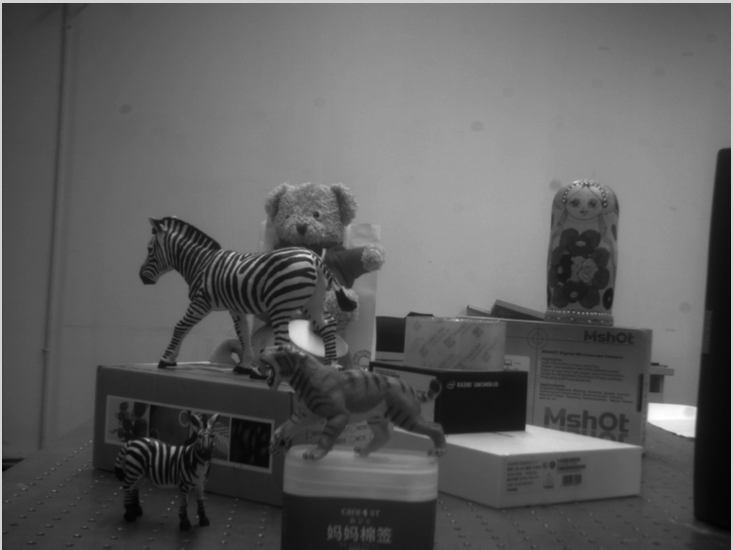
\includegraphics[width=0.45\linewidth]{figure/BETraw}}
            \quad
            \subfigure[$\sigma_2$(最亮处为7,最暗处为0)]{
                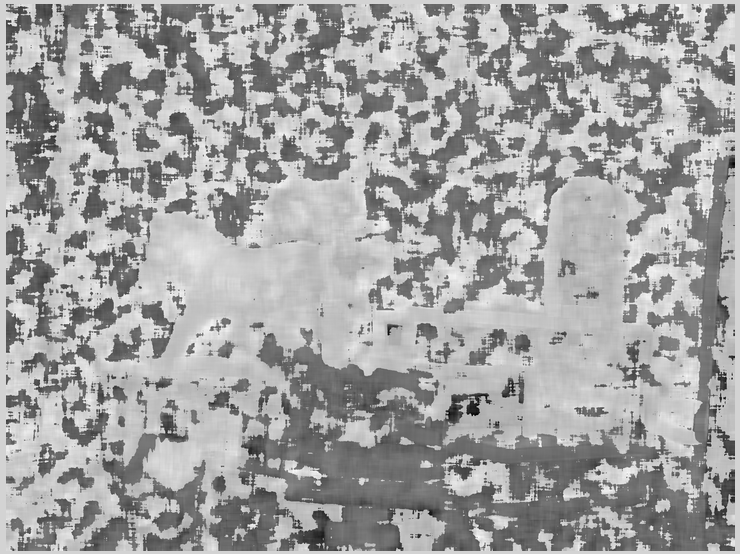
\includegraphics[width=0.45\linewidth]{figure/BETsigma2}}
            \quad
            \subfigure[$blur radius(\sigma = R\sqrt {2}) vs distance$]{
                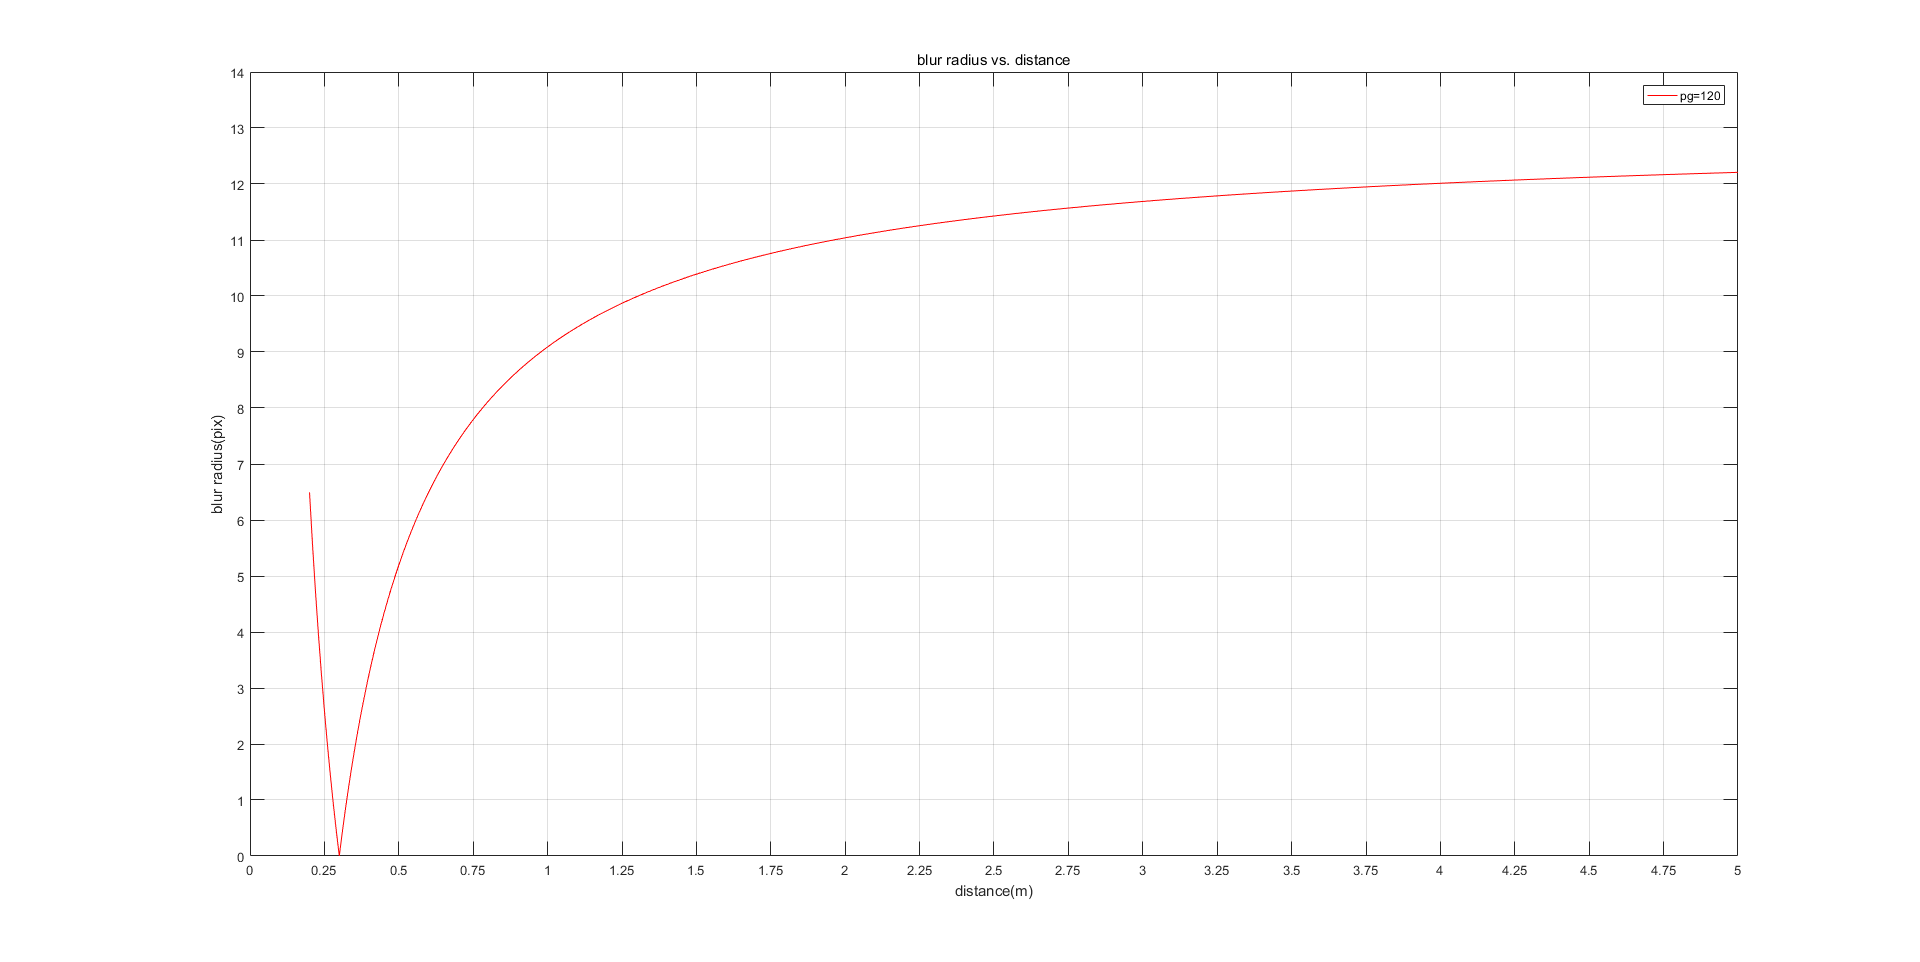
\includegraphics[width=0.9\linewidth]{figure/blurRadiusVsDistance}}
            \quad
            \caption{\small BET效果}
            \label{fig:BET}
        \end{figure}
        \section{基于快速迭代最小化算法的多通道盲去模糊}
        Filip\myciteup{2012Robust}提出基于交替最小化优化策略的盲去卷积算法。该算法利用多通道的数据,将去卷积分为两个步骤:1).$U-Step$图像恢复;2).$H-Step$进行PSF估计;通过TV正则化和基于$R_\Delta$的PSF正则化以及保真项最小化建立优化模型。利用交替乘子法进行迭代优化计算。
        \subsection{U-Step}
        利用H-Step得到的PSF进行图像恢复,其目标函数如式\eqref{eq:mbdUCost},图像运算使用矩阵向量的形式。其中$\left\| Hu-g \right\|^2$ 表征的是保真项,$H$为PSF生成的卷积矩阵。$u$是清晰未退化图像张成的向量,$g$是多个通道模糊图像张成的向量。
        \begin{equation}
            \begin{array}{cc}
                \min\limits_u \frac{\gamma}{2}\left\| Hu-g \right\|^2 +\Phi(D_xu,D_yu)\\
                \Phi(D_xu,D_yu) = \sum\limits_i\sqrt{\left| D_xu\right|^2_i + \left|D_yu\right|^2_i}\\
            \end{array}
            \label{eq:mbdUCost}
        \end{equation}
        将式\eqref{eq:mbdUCost}使用交替方向乘子法做适当松弛之后得到
        \begin{equation}
            \min\limits_{u,v_x,v_y} \mathcal{L}(u,v_x,v_y)= \frac{\gamma}{2}\left\| Hu-g \right\|^2 + \Phi(v_x,v_y) + \frac{\alpha}{2}\left\| D_{x}u-v_x -a_x \right\|^2 + \frac{\alpha}{2}\left\| D_y u -v_y -a_y\right\|^2
        \end{equation}
        其优化算法如下:
        \begin{algorithm}
            \caption{$\hat{u}=u-step(u^0)$}
            \begin{algorithmic}
                \STATE $\bm{Initialization}$: $Set v_x^0=v_y^0=a_x^0=a_y^0=0,\ j = 0$
                \STATE $\bm{Repeat}$:
                \STATE $\bm{Caculate\ u^{j+1} =arg \min\limits_u \mathcal{L}(u,v_x^j,v_y^j) }$:
                \begin{equation}
                    \begin{aligned}
                        u^{j+1} &= A^{-1}\left(H^{T}g +  \frac{\alpha}{\gamma}\left[ D_x^T(v_x^j+a_x^j) + D_y^T(v_y^j+a_y^j) \right]\right)\\
                        A       &= H^{T}H+\frac{\alpha}{\gamma}\left( D^T_xD_x + D^T_yD_y \right)
                    \end{aligned}
                \end{equation}
                \STATE $\bm{Caculate \ {v_x^{j+1}, v_y^{j+1}} = arg \min\limits_{v_x,v_y} \mathcal{L}(u^{j+1},v_x,v_y) }$:
                \begin{equation}
                    \begin{aligned}
                        [v_x^{j+1}]_i &=\left[ D_xu^{j+1}-a^j_x \right]_i[s]_i^-1max([s]_i-\frac{1}{\alpha},0), \\
                        [v_y^{j+1}]_i &=\left[ D_yu^{j+1}-a^j_y \right]_i[s]_i^-1max([s]_i-\frac{1}{\alpha},0), \\
                        [s]_i &= \sqrt {\left[ D_x u^{j+1} - a_x^{j} \right]_i^2 +\left[ D_y u^{j+1} - a_y^{j} \right]_i^2 }\\
                    \end{aligned}
                \end{equation}
                \STATE $\bm{Caculate \ {a_x^{j+1}, a_y^{j+1}} }$:
                \begin{equation}
                    \begin{aligned}
                        a_x^{j+1} &= a_x^{j} - D_xu^{j+1} + v_x^{j+1}\\
                        a_y^{j+1} &= a_y^{j} - D_yu^{j+1} + v_y^{j+1}\\
                    \end{aligned}
                \end{equation}
                \STATE $j = j+1$
                \STATE $\bm{until} \left\| u^{j} - u^{j-1} \right\|/\left\| u^{j} \right\| \leq tol$:
            \end{algorithmic}
            \label{alg:ALM_Ustep}
        \end{algorithm}
        其中对于$H$的构建需要考虑几点:

        \begin{itemize}
            \item 矩阵H的构造,如果构造成普通矩阵,则相关的运算量会巨大,通过构造循环矩阵,可以通过FFT减少运算量;
            \item 如果将H构造成循环矩阵,则需要考虑边界条件,反射填充和常数填充具有不同的效果;
            \item g和u向量需要考虑数据对齐以及边界条件
        \end{itemize}
        循环矩阵(circulant matrix)是一类特殊的toeplitz矩阵,
        \begin{equation}
            C = \begin{pmatrix} z_0    &    z_{n-1}    &    \cdots    & z_1 \\
                    z_1    &    z_0        &    \cdots    & z_2 \\
                    \vdots &    \vdots     &              & \vdots \\
                    z_{n-2}&    z_{n-3}    &    \cdots    & z_{n-1} \\
                    z_{n-1}&    z_{n-2}    &    \cdots    & z_{0} \\
            \end{pmatrix} \triangleq C(z)
            \label{eq:mbcz}
        \end{equation}
        式\eqref{eq:mbcz}可以写成$downshift permutation$矩阵的形式。见式\eqref{eq:mbczl}
        \begin{equation}
            C = \sum\limits_{k=0}^n z_k L^k,\\
            \label{eq:mbczl}
        \end{equation}
        \begin{equation}
            L =
            \left(
            \begin{array}{ccccccccc}
                0      & 0      & \cdots & 0      &       1 \\
                1      & 0      & \cdots & 0      &       0 \\
                0      & 1      & \ddots & 0      &       0 \\
                \vdots &        & \ddots & \ddots &       \vdots\\
                0      & 0      & \cdots & 1      &       0\\
            \end{array}
            \right)\\
            \label{eq:mbl}
        \end{equation}
        利用式\eqref{eq:mbczl}可以简化相关的矩阵运算。对于$h_{mn},u_{MN}$,采用'full'输出的卷积,其输出的大小为$(M+m-1)\times(N+n-1)$,首先将$h$边缘(t,b,l,r)分别填充$(M-1)/2,(N-1)/2$个零。得到$h'$,将$h‘$从中心位置$(M+m-1)/2,(N+n-1)/2$处拆开,张成向量,作为第一列。构成H。同样的现将u的上下左右边界进行填充使其大小和卷积输出大小一致,然后直接张成向量。以$m=n=M=N=3$为例进行说明。张成的H如式\eqref{eq:circulantH}所示。
        \begin{equation}
            h = \begin{pmatrix}
                       h_{00} & h_{01} & h_{02} \\
                       h_{10} & h_{11} & h_{12} \\
                       h_{20} & h_{21} & h_{22} \\
            \end{pmatrix}
        \end{equation}
        \begin{equation}
            h' = \begin{pmatrix}
                           0&    0     &    0   &  0     &  0 \\
                           0&   h_{00} & h_{01} & h_{02} &  0\\
                           0&   h_{10} & h_{11} & h_{12} &  0\\
                           0&   h_{20} & h_{21} & h_{22} &  0\\
                           0&    0     &    0   &  0     &  0 \\
            \end{pmatrix}
        \end{equation}
        \begin{equation}
            \mathcal{H}= \left(   \begin{array}{ccccc|ccccc|ccc|ccccc}
                              h_{11}&   h_{12} &    0   &  0     &  h_{20} &  h_{21} & h_{22} &   0    &   0     &    0   &        & \cdots & h_{00} & h_{01} & h_{02} & 0      & 0      & h_{10}\\
                              h_{10}&   h_{11} & h_{12} &  0     &  0      &  h_{20} & h_{21} & h_{22} &   0     &    0   &        &        &    0   & h_{00} & h_{01} & h_{02} & 0      & 0  \\
                              0&        h_{10} & h_{11} & h_{12} &  0      &   0     & h_{20} & h_{21} & h_{22}  &    0   &        &        &    0   &   0    & h_{00} & h_{01} & h_{02} & 0  \\
                              0&         0     & h_{10} & h_{11} &  h_{12} &   0     &  0     & h_{20} & h_{21}  & h_{22} &        &        &    0   &   0    &  0     & h_{00} & h_{01} & h_{02}  \\
                              h_{02}&    0     &    0   & h_{10} &  h_{11} &   h_{12}&  0     & 0      & h_{20}  & h_{21} & h_{22} &        &    0   &   0    &  0     & 0      & h_{00} & h_{01}  \\
                              \hline
                              h_{01}&   h_{02} &    0   &  0     &  h_{10}      &         &        &        &         &        &        &        &        &        &        &        &        &h_{00}\\
                              h_{00}&   h_{01} & h_{02} &  0     &  0      &         &        &        &         &        &        &        &        &        &        &        &        &\\
                              0     &\\
                             \vdots &\\
                              h_{22}&\\
                              h_{21}&\\
                              h_{20}&\\
                              0     &\\
                              0     &\\
                              h_{12}&\\
            \end{array}\right)
            \label{eq:circulantH}
        \end{equation}
        \begin{equation}
            u = \begin{pmatrix}
                    u_{00} & u_{01} & u_{02} \\
                    u_{10} & u_{11} & u_{12} \\
                    u_{20} & u_{21} & u_{22} \\
            \end{pmatrix}
        \end{equation}
        \begin{equation}
            u' = \begin{pmatrix}
                     0&    0     &    0   &  0     &  0 \\
                     0&   u_{00} & u_{01} & u_{02} &  0\\
                     0&   u_{10} & u_{11} & u_{12} &  0\\
                     0&   u_{20} & u_{21} & u_{22} &  0\\
                     0&    0     &    0   &  0     &  0 \\
            \end{pmatrix}
        \end{equation}
        使用循环矩阵优化的结果如图\ref{fig:ciculantM}其中circulant 表示用循环矩阵构造H(如式\eqref{eq:circulantH})进行计算,BCCB表示用块循环矩阵进行构造H(如式\eqref{eq:bccb})进行计算。bound 0 表示0填充边界,bound 101 表示用镜像填充。
        \begin{figure}[htbp]
            \subfigure[$circulant\ matrix\ bound\ 0\ h1$]{
                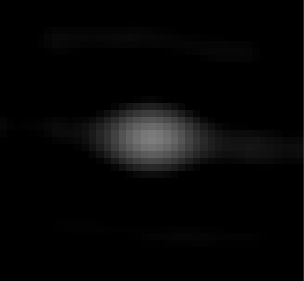
\includegraphics[width=0.3\linewidth]{figure/circulantBound0iter12h1}}
%            \quad
            \subfigure[$circulant\ matrix\ bound\ 0\ h2$]{
                
\includegraphics[width=0.3\linewidth]{figure/circulantBound0iter12h2}}
%            \quad
            \subfigure[$circulant\ matrix\ bound\ 0\ u$]{
                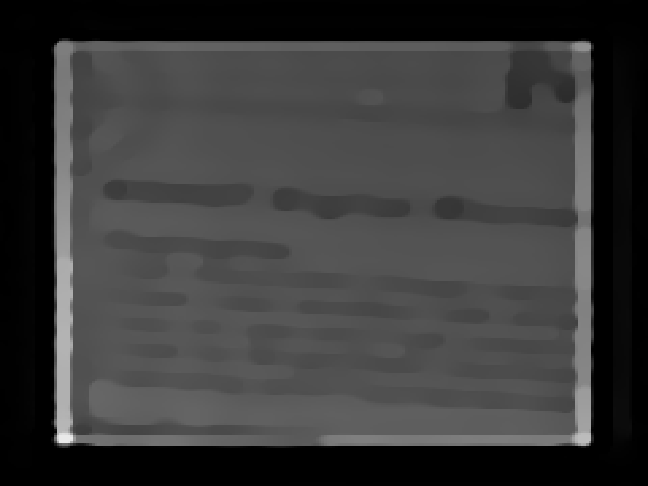
\includegraphics[width=0.3\linewidth]{figure/circulantBound0iter12u}}
%            \quad
            \subfigure[$circulant\ matrix\ bound\ 101\ h1$]{
                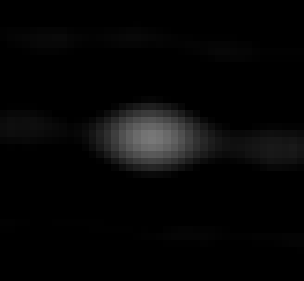
\includegraphics[width=0.3\linewidth]{figure/circulantBound101iter13H1}}
%            \quad
            \subfigure[$circulant\ matrix\ bound\ 101\ h2$]{
                
\includegraphics[width=0.3\linewidth]{figure/circulantBound101iter13h2}}
%            \quad
            \subfigure[$circulant\ matrix\ bound\ 101\ u$]{
                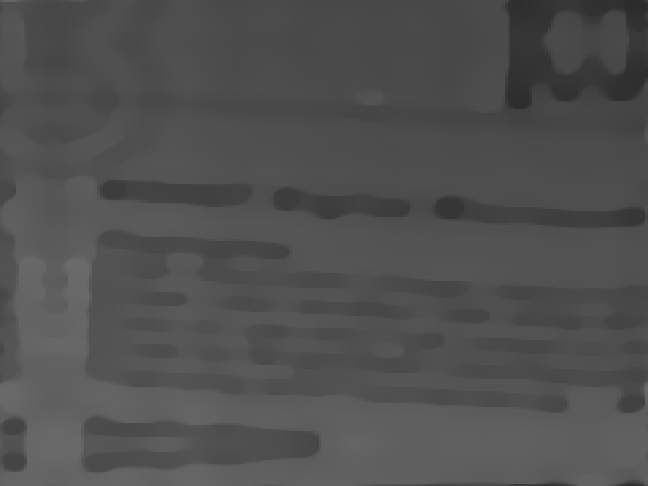
\includegraphics[width=0.3\linewidth]{figure/circulantBound101iter13u}}
%            \quad
            \subfigure[$BCCB\ matrix\ bound\ 101\ h1$]{
                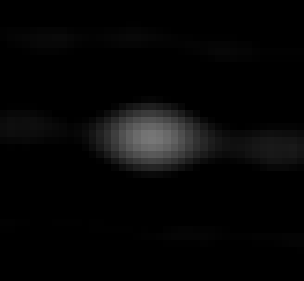
\includegraphics[width=0.3\linewidth]{figure/BCCB_Bound101iter14h1}}
%            \quad
            \subfigure[$BCCB\ matrix\ bound\ 101\ h2$]{
                
\includegraphics[width=0.3\linewidth]{figure/BCCB_Bound101iter14h2}}
%            \quad
            \subfigure[$BCCB\ matrix\ bound\ 101\ u$]{
                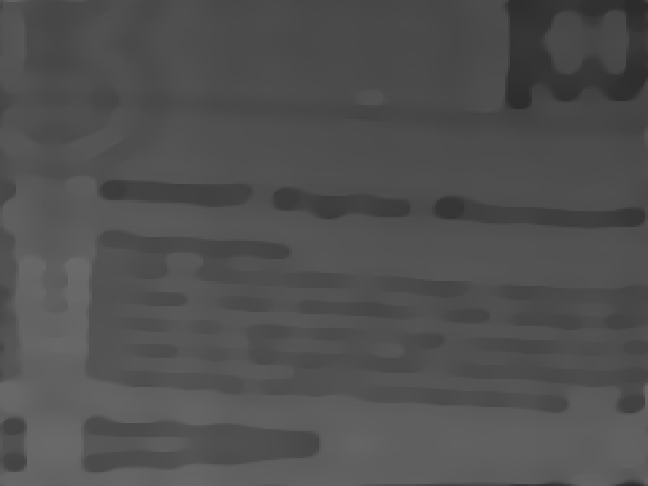
\includegraphics[width=0.3\linewidth]{figure/BCCB_Bound101iter14U}}
%            \quad
            \label{fig:ciculantM}
            \caption{\small 不同矩阵构造和边界效果}
        \end{figure}
        也可以构造块循环矩阵(BCCB,Block circulant matrix with circulant blocks)。
        \begin{equation}
            BCCB = \begin{pmatrix} C_0    &    C_{n-1}    &    \cdots    & C_1 \\
            C_1    &    C_0        &    \cdots    & C_2 \\
            \vdots &    \vdots     &              & \vdots \\
            C_{n-2}&    C_{n-3}    &    \cdots    & C_{n-1} \\
            C_{n-1}&    C_{n-2}    &    \cdots    & C_{0} \\
            \end{pmatrix} \triangleq BCCB(Z)
            \label{eq:mbBccb}
        \end{equation}
        其中$C_i = C(Z(:,i))$。为$Z$的第$i$列生成的循环矩阵。
        利用BCCB来构造可以使用反射边界,从而减少边界的振铃现象。具体构造方法也是先将h填充边界成h’,然后将每行从中间拆开张成向量作为字块的生成向量z,从中间行拆开,组成块循环矩阵,见代码。
        以$m=n=M=N=3$为例进行说明。张成的H如式\eqref{eq:bccb}所示。
        \begin{equation}
            \mathcal{H}= \left(   \begin{array}{ccccc|ccccc|ccc|ccccc}
                                      h_{11}&   h_{12} &    0   &  0     &  h_{10} &  h_{21} & h_{22} &   0    &   0     &h_{20}  & & \cdots &0& h_{01} & h_{02} & 0      & 0      & h_{00}\\
                                      h_{10}&   h_{11} & h_{12} &  0     &  0      &  h_{20} & h_{21} & h_{22} &   0     &    0   & &        &0& h_{00} & h_{01} & h_{02} & 0      & 0  \\
                                      0&        h_{10} & h_{11} & h_{12} &  0      &   0     & h_{20} & h_{21} & h_{22}  &    0   & &        &0&   0    & h_{00} & h_{01} & h_{02} & 0  \\
                                      0&         0     & h_{10} & h_{11} &  h_{12} &   0     &  0     & h_{20} & h_{21}  & h_{22} & &        &0&   0    &  0     & h_{00} & h_{01} & h_{02}  \\
                                      h_{12}&    0     &    0   & h_{10} &  h_{11} &   h_{22}&  0     & 0      & h_{20}  & h_{21} & &        &0& h_{02} &  0     & 0      & h_{00} & h_{01}  \\
                                      \hline
                                      h_{01}&   h_{02} &    0   &  0     &  h_{00}      &         &        &        &         &        &        &        &        &        &        &        &   &0\\
                                      h_{00}&   h_{01} & h_{02} &  0     &  0      &         &        &        &         &        &        &        &        &        &        &        &        &\\
                                      0     &\\
                                      \vdots &\\
                                      h_{22}&\\
                                      h_{21}&\\
                                      h_{20}&\\
                                      0     &\\
                                      0     &\\
                                      h_{22}&\\
            \end{array}\right)
            \label{eq:bccb}
        \end{equation}
    \subsection{H-Step}
        利用$U-Step$得到的恢复好的清晰图像$u$,进行模糊核函数的估算。优化目标函数如式\eqref{eq:mbdHCost}。使用的参数为
        $$\gamma = 1e2;\alpha = 1e-1*gamma; \beta = 1e4*gamma; \delta = 1e3*gamma;maxLoop = 100;tol = 1e-1;$$
        \begin{equation}
            \begin{array}{cc}
                \min\limits_h \mathcal(L)(h) &=  \frac{\gamma}{2}\left\| Uh-g \right\|^2 + \frac{\delta}{2}h^TR_\Delta h + \Psi(h)\\
                R_\Delta = \left[  \Delta G_2 , - \Delta G_1\right]^T\left[  \Delta G_2 , - \Delta G_1\right]\\
                \Psi(h)  = \sum\limits_{k=1}^K\sum\limits_{i=1}^{\hat{L}}\psi(h_k(i)),\psi(t)  =\left\{
                \begin{array}{cc}
                    t, & if \ t \geq 0 \\
                    +\infty,&others\\
                \end{array}
                \right.\\
            \end{array}
            \label{eq:mbdHCost}
        \end{equation}
        利用ALM算法\eqref{eq:mbdHCost}可以转变为\eqref{eq:mbdHwcost}
        \begin{equation}
        \min\limits_h \mathcal{L}(h,w) =  \frac{\gamma}{2}\left\| Uh-g \right\|^2 + \frac{\delta}{2}h^TR_\Delta h + \Psi(w) + \frac{\beta}{2}\left\| h - w - b \right\|^2
            \label{eq:mbdHwcost}
        \end{equation}
        按照如下的优化算法进行迭代求解
        \begin{algorithm}
            \caption{$\hat{h}=h-step(h^0)$}
            \begin{algorithmic}
                \STATE $\bm{Initialization}$: $Set w^0=b^0=0,\ j = 0$
                \STATE $\bm{Repeat}$:
                \STATE $\bm{Caculate\ h^{j+1} =arg \min\limits_u \mathcal{L}(h,w^j) }$:
                \begin{equation}
                    \begin{aligned}
                        h^{j+1} &= B^{-1}\left(U^{T}g +  \frac{\beta}{\gamma}\left[ w^j + b^j \right]\right)\\
                        B       &= U^{T}U+\frac{\delta}{\gamma}R_{\Delta} + \frac{\beta}{\gamma}I
                    \end{aligned}
                \end{equation}
                \STATE $\bm{Caculate \ w^{j+1} = arg \min\limits_{w} \mathcal{L}(h^{j+1},w) }$:
                \begin{equation}
                    \begin{aligned}
                    [w^{j+1}]_i &=max([h^{j+1}-b^j]_i-\frac{1}{\beta},0), \\
                    \end{aligned}
                \end{equation}
                \STATE $\bm{Caculate \ b^{j+1} }$:
                \begin{equation}
                    \begin{aligned}
                        b^{j+1} &= b^{j} - h^{j+1} + w^{j+1}\\
                    \end{aligned}
                \end{equation}
                \STATE $j = j+1$
                \STATE $\bm{until} \left\| h^{j} - h^{j-1} \right\|/\left\| h^{j} \right\| \leq tol$:
            \end{algorithmic}
            \label{alg:ALM_Hstep}
        \end{algorithm}
        需要注意一下几点:
        \begin{itemize}
            \item $U,R_\Delta$ 的构造需要考虑不同卷积输出模式的影响,论文推荐的是valid模式
            \item $U,R_\Delta$矩阵相关运算,可以使用FFT运算加速,代码中使用的是opencv的API \ matchTemplate(内部已经用fft做了优化)
            \item 进行相关的处理之前,需要对图像进行预处理,代码中实现的预处理包括用一个比较小的高斯核进行滤波,进行归一化
        \end{itemize}
        \subsection{实验结果}
        实验结果见图\ref{fig:mbdResult},其中第一行的图片是迭代处理后的图像和psf,第二行是原始的图片$(g1+g2)/2$,以及根据实际情况大致预测的PSF。图示总计迭代了6次,参数为
        $$
        L = 41,
        image size = 256,
        \gamma = 1e2,
        \alpha = 1e0*\gamma,
        \beta = 1e4*\gamma,
        \delta = 1e3*\gamma,
        $$
        \begin{figure}[htbp]
            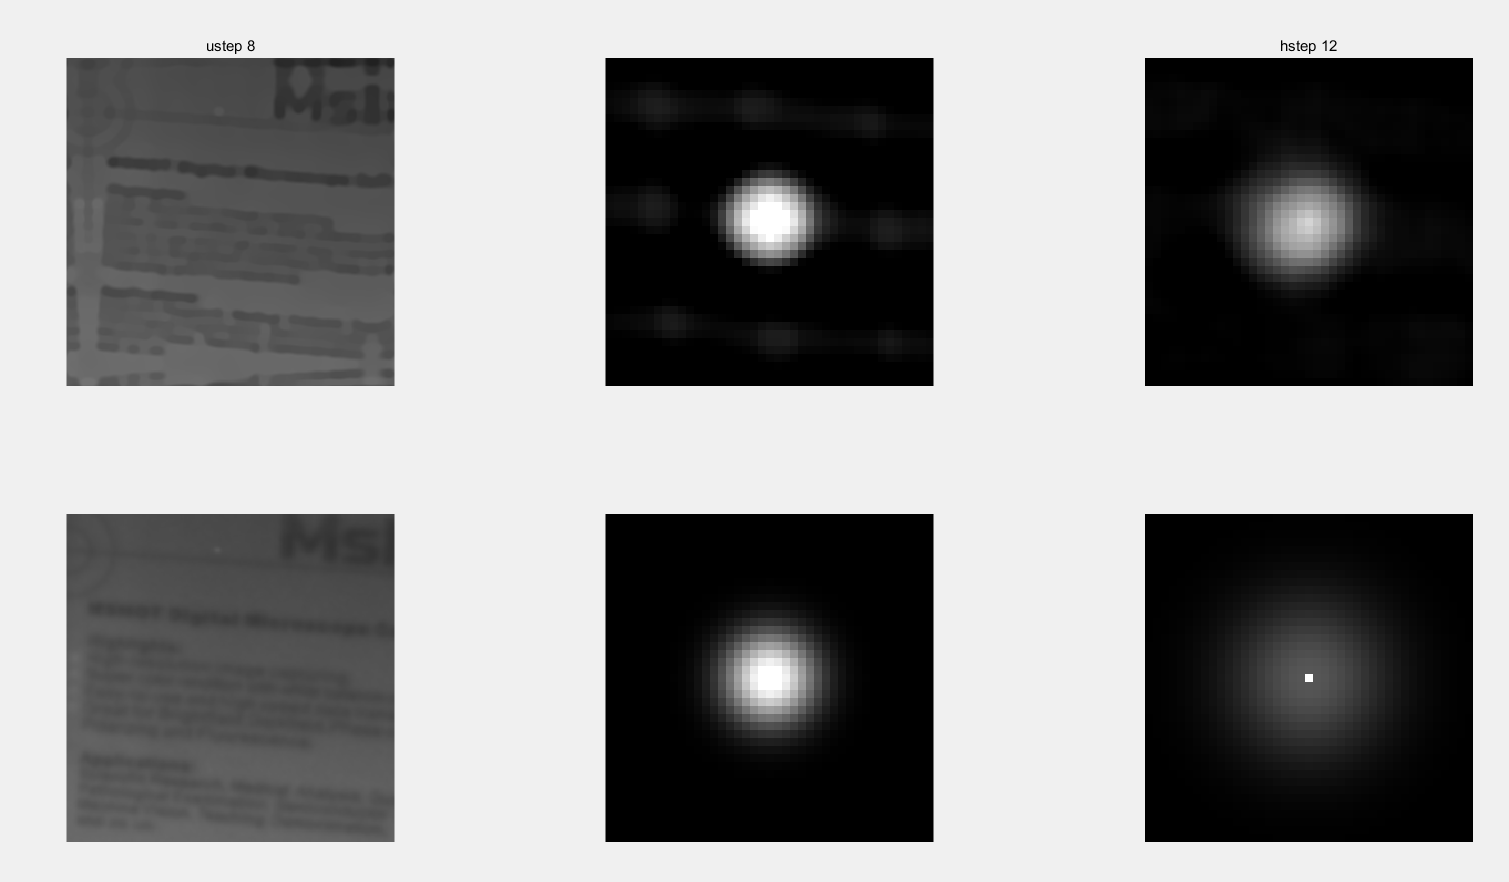
\includegraphics[width=0.9\linewidth]{figure/MBD}
            \label{fig:mbdResult}
        \end{figure}
        \section{接下来的工作}
        \begin{itemize}
            \item 进一步完善MBD算法的实验,考虑使用TGV进行图像恢复
            \item 复现wild dfd
        \end{itemize}




        \bibliography{main}
        \bibliographystyle{plain}
    \end{sloppypar}

\end{document}
